\documentclass[11pt]{article}
\newcommand{\LabNumber}{1}
\newcommand{\LabTitle}{ROM as Control Store}
\newcommand{\LabTopic}{A microprocessor with no instruction register and no opcode decode -- the ROM word \emph{is} the control word}
\newcommand{\LabDuration}{2 hours (in-lab)}
% Shared preamble for Computer Programming lab sheets.
% Include with % Shared preamble for Computer Programming lab sheets.
% Include with % Shared preamble for Computer Programming lab sheets.
% Include with \input{common.tex} after \documentclass{article}.

\usepackage[a4paper,margin=2.2cm]{geometry}
\usepackage[T1]{fontenc}
\usepackage{lmodern}
\usepackage{microtype}
\usepackage{enumitem}
\usepackage{xcolor}
\usepackage{tcolorbox}
\tcbuselibrary{breakable,skins}
\usepackage{listings}
\usepackage{fancyhdr}
\usepackage{titlesec}
\usepackage{amsmath}
\usepackage{array}
\usepackage{booktabs}
\usepackage{hyperref}

\hypersetup{
  colorlinks=true,
  linkcolor=black,
  urlcolor=blue!60!black,
  pdfborder={0 0 0}
}

% ---------- Course identity (override per file if needed) ----------
\providecommand{\CourseName}{Microprocessors}
\providecommand{\CourseCode}{010153521}
\providecommand{\Semester}{Semester 1/2026}
\providecommand{\LabDuration}{3 hours (in-lab)}

% ---------- Colors ----------
\definecolor{accent}{HTML}{1F4E79}
\definecolor{accentlight}{HTML}{D9E2EC}
\definecolor{warn}{HTML}{B45309}
\definecolor{ok}{HTML}{166534}
\definecolor{codebg}{HTML}{F6F8FA}
\definecolor{codeframe}{HTML}{D0D7DE}
\definecolor{codekw}{HTML}{0550AE}
\definecolor{codestr}{HTML}{0A7B2C}
\definecolor{codecom}{HTML}{6E7781}

% ---------- Code / assembly listings ----------
\lstdefinestyle{c}{
  language=C,
  basicstyle=\ttfamily\small,
  keywordstyle=\color{codekw}\bfseries,
  stringstyle=\color{codestr},
  commentstyle=\color{codecom}\itshape,
  backgroundcolor=\color{codebg},
  frame=single,
  rulecolor=\color{codeframe},
  framerule=0.4pt,
  showstringspaces=false,
  breaklines=true,
  columns=fullflexible,
  keepspaces=true,
  tabsize=4,
  xleftmargin=8pt,
  xrightmargin=4pt,
  aboveskip=6pt,
  belowskip=6pt,
}
\lstdefinestyle{asm}{
  basicstyle=\ttfamily\small,
  commentstyle=\color{codecom}\itshape,
  backgroundcolor=\color{codebg},
  frame=single,
  rulecolor=\color{codeframe},
  framerule=0.4pt,
  showstringspaces=false,
  breaklines=true,
  columns=fullflexible,
  keepspaces=true,
  tabsize=4,
  xleftmargin=8pt,
  xrightmargin=4pt,
  aboveskip=6pt,
  belowskip=6pt,
}
\lstset{style=asm}

% ---------- Section styling ----------
\titleformat{\section}{\Large\bfseries\color{accent}}{\thesection.}{0.5em}{}
\titleformat{\subsection}{\large\bfseries\color{accent!85!black}}{\thesubsection}{0.5em}{}
\titlespacing*{\section}{0pt}{12pt}{6pt}
\titlespacing*{\subsection}{0pt}{8pt}{4pt}

% ---------- Page headers/footers ----------
\pagestyle{fancy}
\fancyhf{}
\fancyhead[L]{\small\CourseName\ifx\CourseCode\empty\else\ (\CourseCode)\fi}
\fancyhead[C]{\small\Semester}
\fancyhead[R]{\small\textbf{Lab \LabNumber:} \LabTitle}
\fancyfoot[C]{\small\thepage}
\renewcommand{\headrulewidth}{0.4pt}

% ---------- Title block ----------
\newcommand{\labheader}{%
  \begin{tcolorbox}[
    enhanced,
    colback=accentlight,
    colframe=accent,
    boxrule=0.5pt,
    arc=2pt,
    left=10pt, right=10pt, top=8pt, bottom=8pt
  ]
    {\Large\bfseries\color{accent} Lab \LabNumber: \LabTitle}\\[2pt]
    {\small \CourseName\ifx\CourseCode\empty\else\ (\CourseCode)\fi\quad\textbar\quad \Semester}\\[1pt]
    {\small \textbf{Duration:} \LabDuration\quad\textbar\quad \textbf{Topic:} \LabTopic}
  \end{tcolorbox}
  \vspace{2pt}
}

% ---------- Custom environments ----------
\newtcolorbox{summary}[1][Quick Reference]{
  enhanced,breakable,
  colback=accentlight!40,colframe=accent!70,
  title={\bfseries #1},
  fonttitle=\color{white},
  attach boxed title to top left={xshift=6pt,yshift=-3pt},
  boxed title style={colback=accent,boxrule=0pt,arc=2pt},
  arc=2pt,boxrule=0.4pt,
  top=12pt,
}

\newcounter{labex}[section]
\newtcolorbox{labexercise}[1]{
  enhanced,breakable,
  colback=white,colframe=accent,
  title={\bfseries In-Lab Exercise \refstepcounter{labex}\thelabex: #1},
  fonttitle=\color{white},
  attach boxed title to top left={xshift=6pt,yshift=-3pt},
  boxed title style={colback=accent,boxrule=0pt,arc=2pt},
  arc=2pt,boxrule=0.4pt,
  top=12pt,
}

\newcounter{traceex}
\newtcolorbox{trace}[1][]{
  enhanced,breakable,
  colback=white,colframe=warn,
  title={\bfseries Trace \& Predict \refstepcounter{traceex}\thetraceex\ifx\\#1\\\else: #1\fi},
  fonttitle=\color{white},
  attach boxed title to top left={xshift=6pt,yshift=-3pt},
  boxed title style={colback=warn,boxrule=0pt,arc=2pt},
  arc=2pt,boxrule=0.4pt,
  top=12pt,
}

\newcounter{bugex}
\newtcolorbox{bug}[1][]{
  enhanced,breakable,
  colback=white,colframe=warn,
  title={\bfseries Find the Bug \refstepcounter{bugex}\thebugex\ifx\\#1\\\else: #1\fi},
  fonttitle=\color{white},
  attach boxed title to top left={xshift=6pt,yshift=-3pt},
  boxed title style={colback=warn,boxrule=0pt,arc=2pt},
  arc=2pt,boxrule=0.4pt,
  top=12pt,
}

\newcounter{writeex}
\newtcolorbox{writecode}[1][]{
  enhanced,breakable,
  colback=white,colframe=warn,
  title={\bfseries Write Code on Paper \refstepcounter{writeex}\thewriteex\ifx\\#1\\\else: #1\fi},
  fonttitle=\color{white},
  attach boxed title to top left={xshift=6pt,yshift=-3pt},
  boxed title style={colback=warn,boxrule=0pt,arc=2pt},
  arc=2pt,boxrule=0.4pt,
  top=12pt,
}

% ---------- AI Collaboration box ----------
\definecolor{aipurple}{HTML}{4C1D95}
\definecolor{aipurplelight}{HTML}{EDE9FE}

\newtcolorbox{aicollab}[1][AI Collaboration]{
  enhanced,breakable,
  colback=aipurplelight,colframe=aipurple!70,
  title={\bfseries #1},
  fonttitle=\color{white},
  attach boxed title to top left={xshift=6pt,yshift=-3pt},
  boxed title style={colback=aipurple,boxrule=0pt,arc=2pt},
  arc=2pt,boxrule=0.4pt,
  top=12pt,
}

\newcounter{tryex}
\newtcolorbox{tryit}[1]{
  enhanced,breakable,
  colback=ok!6,colframe=ok!70!black,
  title={\bfseries Try It \refstepcounter{tryex}\thetryex: #1},
  fonttitle=\color{white},
  attach boxed title to top left={xshift=6pt,yshift=-3pt},
  boxed title style={colback=ok!70!black,boxrule=0pt,arc=2pt},
  arc=2pt,boxrule=0.4pt,
  top=12pt,
}

% ---------- Drawing exercise ----------
\definecolor{drawteal}{HTML}{0D7377}
\definecolor{drawteallight}{HTML}{D4F1F4}

\newcounter{drawex}
\newtcolorbox{drawex}[1]{
  enhanced,breakable,
  colback=drawteallight,colframe=drawteal!70,
  title={\bfseries Draw on Paper \refstepcounter{drawex}\thedrawex: #1},
  fonttitle=\color{white},
  attach boxed title to top left={xshift=6pt,yshift=-3pt},
  boxed title style={colback=drawteal,boxrule=0pt,arc=2pt},
  arc=2pt,boxrule=0.4pt,
  top=12pt,
}


\newcommand{\takehomebanner}{%
  \vspace{6pt}
  \begin{tcolorbox}[
    colback=warn!10,colframe=warn,boxrule=0.5pt,arc=2pt,
    left=10pt,right=10pt,top=6pt,bottom=6pt
  ]
    \textbf{Take-Home (Paper Work).}\;
    Solve the following on paper without using a computer or compiler.
    Hand-write your answers; submit at the start of the next lab.
    Goal: prepare you to dry-code during the written exam.
  \end{tcolorbox}
  \vspace{4pt}
}
 after \documentclass{article}.

\usepackage[a4paper,margin=2.2cm]{geometry}
\usepackage[T1]{fontenc}
\usepackage{lmodern}
\usepackage{microtype}
\usepackage{enumitem}
\usepackage{xcolor}
\usepackage{tcolorbox}
\tcbuselibrary{breakable,skins}
\usepackage{listings}
\usepackage{fancyhdr}
\usepackage{titlesec}
\usepackage{amsmath}
\usepackage{array}
\usepackage{booktabs}
\usepackage{hyperref}

\hypersetup{
  colorlinks=true,
  linkcolor=black,
  urlcolor=blue!60!black,
  pdfborder={0 0 0}
}

% ---------- Course identity (override per file if needed) ----------
\providecommand{\CourseName}{Microprocessors}
\providecommand{\CourseCode}{010153521}
\providecommand{\Semester}{Semester 1/2026}
\providecommand{\LabDuration}{3 hours (in-lab)}

% ---------- Colors ----------
\definecolor{accent}{HTML}{1F4E79}
\definecolor{accentlight}{HTML}{D9E2EC}
\definecolor{warn}{HTML}{B45309}
\definecolor{ok}{HTML}{166534}
\definecolor{codebg}{HTML}{F6F8FA}
\definecolor{codeframe}{HTML}{D0D7DE}
\definecolor{codekw}{HTML}{0550AE}
\definecolor{codestr}{HTML}{0A7B2C}
\definecolor{codecom}{HTML}{6E7781}

% ---------- Code / assembly listings ----------
\lstdefinestyle{c}{
  language=C,
  basicstyle=\ttfamily\small,
  keywordstyle=\color{codekw}\bfseries,
  stringstyle=\color{codestr},
  commentstyle=\color{codecom}\itshape,
  backgroundcolor=\color{codebg},
  frame=single,
  rulecolor=\color{codeframe},
  framerule=0.4pt,
  showstringspaces=false,
  breaklines=true,
  columns=fullflexible,
  keepspaces=true,
  tabsize=4,
  xleftmargin=8pt,
  xrightmargin=4pt,
  aboveskip=6pt,
  belowskip=6pt,
}
\lstdefinestyle{asm}{
  basicstyle=\ttfamily\small,
  commentstyle=\color{codecom}\itshape,
  backgroundcolor=\color{codebg},
  frame=single,
  rulecolor=\color{codeframe},
  framerule=0.4pt,
  showstringspaces=false,
  breaklines=true,
  columns=fullflexible,
  keepspaces=true,
  tabsize=4,
  xleftmargin=8pt,
  xrightmargin=4pt,
  aboveskip=6pt,
  belowskip=6pt,
}
\lstset{style=asm}

% ---------- Section styling ----------
\titleformat{\section}{\Large\bfseries\color{accent}}{\thesection.}{0.5em}{}
\titleformat{\subsection}{\large\bfseries\color{accent!85!black}}{\thesubsection}{0.5em}{}
\titlespacing*{\section}{0pt}{12pt}{6pt}
\titlespacing*{\subsection}{0pt}{8pt}{4pt}

% ---------- Page headers/footers ----------
\pagestyle{fancy}
\fancyhf{}
\fancyhead[L]{\small\CourseName\ifx\CourseCode\empty\else\ (\CourseCode)\fi}
\fancyhead[C]{\small\Semester}
\fancyhead[R]{\small\textbf{Lab \LabNumber:} \LabTitle}
\fancyfoot[C]{\small\thepage}
\renewcommand{\headrulewidth}{0.4pt}

% ---------- Title block ----------
\newcommand{\labheader}{%
  \begin{tcolorbox}[
    enhanced,
    colback=accentlight,
    colframe=accent,
    boxrule=0.5pt,
    arc=2pt,
    left=10pt, right=10pt, top=8pt, bottom=8pt
  ]
    {\Large\bfseries\color{accent} Lab \LabNumber: \LabTitle}\\[2pt]
    {\small \CourseName\ifx\CourseCode\empty\else\ (\CourseCode)\fi\quad\textbar\quad \Semester}\\[1pt]
    {\small \textbf{Duration:} \LabDuration\quad\textbar\quad \textbf{Topic:} \LabTopic}
  \end{tcolorbox}
  \vspace{2pt}
}

% ---------- Custom environments ----------
\newtcolorbox{summary}[1][Quick Reference]{
  enhanced,breakable,
  colback=accentlight!40,colframe=accent!70,
  title={\bfseries #1},
  fonttitle=\color{white},
  attach boxed title to top left={xshift=6pt,yshift=-3pt},
  boxed title style={colback=accent,boxrule=0pt,arc=2pt},
  arc=2pt,boxrule=0.4pt,
  top=12pt,
}

\newcounter{labex}[section]
\newtcolorbox{labexercise}[1]{
  enhanced,breakable,
  colback=white,colframe=accent,
  title={\bfseries In-Lab Exercise \refstepcounter{labex}\thelabex: #1},
  fonttitle=\color{white},
  attach boxed title to top left={xshift=6pt,yshift=-3pt},
  boxed title style={colback=accent,boxrule=0pt,arc=2pt},
  arc=2pt,boxrule=0.4pt,
  top=12pt,
}

\newcounter{traceex}
\newtcolorbox{trace}[1][]{
  enhanced,breakable,
  colback=white,colframe=warn,
  title={\bfseries Trace \& Predict \refstepcounter{traceex}\thetraceex\ifx\\#1\\\else: #1\fi},
  fonttitle=\color{white},
  attach boxed title to top left={xshift=6pt,yshift=-3pt},
  boxed title style={colback=warn,boxrule=0pt,arc=2pt},
  arc=2pt,boxrule=0.4pt,
  top=12pt,
}

\newcounter{bugex}
\newtcolorbox{bug}[1][]{
  enhanced,breakable,
  colback=white,colframe=warn,
  title={\bfseries Find the Bug \refstepcounter{bugex}\thebugex\ifx\\#1\\\else: #1\fi},
  fonttitle=\color{white},
  attach boxed title to top left={xshift=6pt,yshift=-3pt},
  boxed title style={colback=warn,boxrule=0pt,arc=2pt},
  arc=2pt,boxrule=0.4pt,
  top=12pt,
}

\newcounter{writeex}
\newtcolorbox{writecode}[1][]{
  enhanced,breakable,
  colback=white,colframe=warn,
  title={\bfseries Write Code on Paper \refstepcounter{writeex}\thewriteex\ifx\\#1\\\else: #1\fi},
  fonttitle=\color{white},
  attach boxed title to top left={xshift=6pt,yshift=-3pt},
  boxed title style={colback=warn,boxrule=0pt,arc=2pt},
  arc=2pt,boxrule=0.4pt,
  top=12pt,
}

% ---------- AI Collaboration box ----------
\definecolor{aipurple}{HTML}{4C1D95}
\definecolor{aipurplelight}{HTML}{EDE9FE}

\newtcolorbox{aicollab}[1][AI Collaboration]{
  enhanced,breakable,
  colback=aipurplelight,colframe=aipurple!70,
  title={\bfseries #1},
  fonttitle=\color{white},
  attach boxed title to top left={xshift=6pt,yshift=-3pt},
  boxed title style={colback=aipurple,boxrule=0pt,arc=2pt},
  arc=2pt,boxrule=0.4pt,
  top=12pt,
}

\newcounter{tryex}
\newtcolorbox{tryit}[1]{
  enhanced,breakable,
  colback=ok!6,colframe=ok!70!black,
  title={\bfseries Try It \refstepcounter{tryex}\thetryex: #1},
  fonttitle=\color{white},
  attach boxed title to top left={xshift=6pt,yshift=-3pt},
  boxed title style={colback=ok!70!black,boxrule=0pt,arc=2pt},
  arc=2pt,boxrule=0.4pt,
  top=12pt,
}

% ---------- Drawing exercise ----------
\definecolor{drawteal}{HTML}{0D7377}
\definecolor{drawteallight}{HTML}{D4F1F4}

\newcounter{drawex}
\newtcolorbox{drawex}[1]{
  enhanced,breakable,
  colback=drawteallight,colframe=drawteal!70,
  title={\bfseries Draw on Paper \refstepcounter{drawex}\thedrawex: #1},
  fonttitle=\color{white},
  attach boxed title to top left={xshift=6pt,yshift=-3pt},
  boxed title style={colback=drawteal,boxrule=0pt,arc=2pt},
  arc=2pt,boxrule=0.4pt,
  top=12pt,
}


\newcommand{\takehomebanner}{%
  \vspace{6pt}
  \begin{tcolorbox}[
    colback=warn!10,colframe=warn,boxrule=0.5pt,arc=2pt,
    left=10pt,right=10pt,top=6pt,bottom=6pt
  ]
    \textbf{Take-Home (Paper Work).}\;
    Solve the following on paper without using a computer or compiler.
    Hand-write your answers; submit at the start of the next lab.
    Goal: prepare you to dry-code during the written exam.
  \end{tcolorbox}
  \vspace{4pt}
}
 after \documentclass{article}.

\usepackage[a4paper,margin=2.2cm]{geometry}
\usepackage[T1]{fontenc}
\usepackage{lmodern}
\usepackage{microtype}
\usepackage{enumitem}
\usepackage{xcolor}
\usepackage{tcolorbox}
\tcbuselibrary{breakable,skins}
\usepackage{listings}
\usepackage{fancyhdr}
\usepackage{titlesec}
\usepackage{amsmath}
\usepackage{array}
\usepackage{booktabs}
\usepackage{hyperref}

\hypersetup{
  colorlinks=true,
  linkcolor=black,
  urlcolor=blue!60!black,
  pdfborder={0 0 0}
}

% ---------- Course identity (override per file if needed) ----------
\providecommand{\CourseName}{Microprocessors}
\providecommand{\CourseCode}{010153521}
\providecommand{\Semester}{Semester 1/2026}
\providecommand{\LabDuration}{3 hours (in-lab)}

% ---------- Colors ----------
\definecolor{accent}{HTML}{1F4E79}
\definecolor{accentlight}{HTML}{D9E2EC}
\definecolor{warn}{HTML}{B45309}
\definecolor{ok}{HTML}{166534}
\definecolor{codebg}{HTML}{F6F8FA}
\definecolor{codeframe}{HTML}{D0D7DE}
\definecolor{codekw}{HTML}{0550AE}
\definecolor{codestr}{HTML}{0A7B2C}
\definecolor{codecom}{HTML}{6E7781}

% ---------- Code / assembly listings ----------
\lstdefinestyle{c}{
  language=C,
  basicstyle=\ttfamily\small,
  keywordstyle=\color{codekw}\bfseries,
  stringstyle=\color{codestr},
  commentstyle=\color{codecom}\itshape,
  backgroundcolor=\color{codebg},
  frame=single,
  rulecolor=\color{codeframe},
  framerule=0.4pt,
  showstringspaces=false,
  breaklines=true,
  columns=fullflexible,
  keepspaces=true,
  tabsize=4,
  xleftmargin=8pt,
  xrightmargin=4pt,
  aboveskip=6pt,
  belowskip=6pt,
}
\lstdefinestyle{asm}{
  basicstyle=\ttfamily\small,
  commentstyle=\color{codecom}\itshape,
  backgroundcolor=\color{codebg},
  frame=single,
  rulecolor=\color{codeframe},
  framerule=0.4pt,
  showstringspaces=false,
  breaklines=true,
  columns=fullflexible,
  keepspaces=true,
  tabsize=4,
  xleftmargin=8pt,
  xrightmargin=4pt,
  aboveskip=6pt,
  belowskip=6pt,
}
\lstset{style=asm}

% ---------- Section styling ----------
\titleformat{\section}{\Large\bfseries\color{accent}}{\thesection.}{0.5em}{}
\titleformat{\subsection}{\large\bfseries\color{accent!85!black}}{\thesubsection}{0.5em}{}
\titlespacing*{\section}{0pt}{12pt}{6pt}
\titlespacing*{\subsection}{0pt}{8pt}{4pt}

% ---------- Page headers/footers ----------
\pagestyle{fancy}
\fancyhf{}
\fancyhead[L]{\small\CourseName\ifx\CourseCode\empty\else\ (\CourseCode)\fi}
\fancyhead[C]{\small\Semester}
\fancyhead[R]{\small\textbf{Lab \LabNumber:} \LabTitle}
\fancyfoot[C]{\small\thepage}
\renewcommand{\headrulewidth}{0.4pt}

% ---------- Title block ----------
\newcommand{\labheader}{%
  \begin{tcolorbox}[
    enhanced,
    colback=accentlight,
    colframe=accent,
    boxrule=0.5pt,
    arc=2pt,
    left=10pt, right=10pt, top=8pt, bottom=8pt
  ]
    {\Large\bfseries\color{accent} Lab \LabNumber: \LabTitle}\\[2pt]
    {\small \CourseName\ifx\CourseCode\empty\else\ (\CourseCode)\fi\quad\textbar\quad \Semester}\\[1pt]
    {\small \textbf{Duration:} \LabDuration\quad\textbar\quad \textbf{Topic:} \LabTopic}
  \end{tcolorbox}
  \vspace{2pt}
}

% ---------- Custom environments ----------
\newtcolorbox{summary}[1][Quick Reference]{
  enhanced,breakable,
  colback=accentlight!40,colframe=accent!70,
  title={\bfseries #1},
  fonttitle=\color{white},
  attach boxed title to top left={xshift=6pt,yshift=-3pt},
  boxed title style={colback=accent,boxrule=0pt,arc=2pt},
  arc=2pt,boxrule=0.4pt,
  top=12pt,
}

\newcounter{labex}[section]
\newtcolorbox{labexercise}[1]{
  enhanced,breakable,
  colback=white,colframe=accent,
  title={\bfseries In-Lab Exercise \refstepcounter{labex}\thelabex: #1},
  fonttitle=\color{white},
  attach boxed title to top left={xshift=6pt,yshift=-3pt},
  boxed title style={colback=accent,boxrule=0pt,arc=2pt},
  arc=2pt,boxrule=0.4pt,
  top=12pt,
}

\newcounter{traceex}
\newtcolorbox{trace}[1][]{
  enhanced,breakable,
  colback=white,colframe=warn,
  title={\bfseries Trace \& Predict \refstepcounter{traceex}\thetraceex\ifx\\#1\\\else: #1\fi},
  fonttitle=\color{white},
  attach boxed title to top left={xshift=6pt,yshift=-3pt},
  boxed title style={colback=warn,boxrule=0pt,arc=2pt},
  arc=2pt,boxrule=0.4pt,
  top=12pt,
}

\newcounter{bugex}
\newtcolorbox{bug}[1][]{
  enhanced,breakable,
  colback=white,colframe=warn,
  title={\bfseries Find the Bug \refstepcounter{bugex}\thebugex\ifx\\#1\\\else: #1\fi},
  fonttitle=\color{white},
  attach boxed title to top left={xshift=6pt,yshift=-3pt},
  boxed title style={colback=warn,boxrule=0pt,arc=2pt},
  arc=2pt,boxrule=0.4pt,
  top=12pt,
}

\newcounter{writeex}
\newtcolorbox{writecode}[1][]{
  enhanced,breakable,
  colback=white,colframe=warn,
  title={\bfseries Write Code on Paper \refstepcounter{writeex}\thewriteex\ifx\\#1\\\else: #1\fi},
  fonttitle=\color{white},
  attach boxed title to top left={xshift=6pt,yshift=-3pt},
  boxed title style={colback=warn,boxrule=0pt,arc=2pt},
  arc=2pt,boxrule=0.4pt,
  top=12pt,
}

% ---------- AI Collaboration box ----------
\definecolor{aipurple}{HTML}{4C1D95}
\definecolor{aipurplelight}{HTML}{EDE9FE}

\newtcolorbox{aicollab}[1][AI Collaboration]{
  enhanced,breakable,
  colback=aipurplelight,colframe=aipurple!70,
  title={\bfseries #1},
  fonttitle=\color{white},
  attach boxed title to top left={xshift=6pt,yshift=-3pt},
  boxed title style={colback=aipurple,boxrule=0pt,arc=2pt},
  arc=2pt,boxrule=0.4pt,
  top=12pt,
}

\newcounter{tryex}
\newtcolorbox{tryit}[1]{
  enhanced,breakable,
  colback=ok!6,colframe=ok!70!black,
  title={\bfseries Try It \refstepcounter{tryex}\thetryex: #1},
  fonttitle=\color{white},
  attach boxed title to top left={xshift=6pt,yshift=-3pt},
  boxed title style={colback=ok!70!black,boxrule=0pt,arc=2pt},
  arc=2pt,boxrule=0.4pt,
  top=12pt,
}

% ---------- Drawing exercise ----------
\definecolor{drawteal}{HTML}{0D7377}
\definecolor{drawteallight}{HTML}{D4F1F4}

\newcounter{drawex}
\newtcolorbox{drawex}[1]{
  enhanced,breakable,
  colback=drawteallight,colframe=drawteal!70,
  title={\bfseries Draw on Paper \refstepcounter{drawex}\thedrawex: #1},
  fonttitle=\color{white},
  attach boxed title to top left={xshift=6pt,yshift=-3pt},
  boxed title style={colback=drawteal,boxrule=0pt,arc=2pt},
  arc=2pt,boxrule=0.4pt,
  top=12pt,
}


\newcommand{\takehomebanner}{%
  \vspace{6pt}
  \begin{tcolorbox}[
    colback=warn!10,colframe=warn,boxrule=0.5pt,arc=2pt,
    left=10pt,right=10pt,top=6pt,bottom=6pt
  ]
    \textbf{Take-Home (Paper Work).}\;
    Solve the following on paper without using a computer or compiler.
    Hand-write your answers; submit at the start of the next lab.
    Goal: prepare you to dry-code during the written exam.
  \end{tcolorbox}
  \vspace{4pt}
}

\usepackage{amssymb}
\usepackage{graphicx}

\begin{document}
\labheader

\section*{Objectives}
\begin{itemize}[leftmargin=*,nosep]
  \item Explain the difference between a \emph{control-word} machine (this lab,
        where every ROM bit \emph{is} a control signal directly -- there is no
        opcode, no Instruction Register, and no decode step at all) and a
        \emph{hardwired FSM} control unit (Lab 2's EC-1, which decodes an
        opcode into signals).
  \item Build a self-addressing program counter: a register that feeds its own next
        value back from either an incrementer or a ROM-supplied jump address.
  \item Design the small piece of glue logic that sits \emph{between} the ROM and the
        PC and decides, every cycle, whether to jump.
  \item Hand-assemble a control-word microprogram, load it into ROM, and verify a
        0-to-10 counting sequence cycle by cycle.
\end{itemize}

\begin{summary}[Quick Reference: The Control Word]
Program memory is 16 $\times$ 8-bit ROM. Unlike EC-1, there is \textbf{no opcode and
no operand split} -- every one of the 8 bits drives something directly:
\begin{center}
\begin{tabular}{@{}cccccccc@{}}
\toprule
\multicolumn{4}{c}{bit 7 \quad\ldots\quad bit 4} & \multicolumn{4}{c}{bit 3 \quad\ldots\quad bit 0} \\
\midrule
\texttt{SEQ} & \texttt{LD\_A} & \texttt{CLR\_A} & \texttt{OUT} & \multicolumn{4}{c}{\texttt{ADDR[3:0]}} \\
\bottomrule
\end{tabular}
\end{center}
\texttt{LD\_A}, \texttt{CLR\_A}, \texttt{OUT} drive the Accumulator side directly.
\texttt{ADDR[3:0]} is a jump target -- meaningful only when \texttt{SEQ=0}.
\texttt{SEQ=1} means ``ignore \texttt{ADDR}, just advance to \texttt{PC+1}.''
There is one piece of logic \emph{outside} the ROM, sitting between it and the PC:
\[
\texttt{PC\_load} = \overline{\texttt{SEQ}} \cdot (\texttt{OUT} + \texttt{NEQ\_10})
\]
where \texttt{NEQ\_10} is a comparator flag ($=1$ when \texttt{ACC} $\neq 10$).
When \texttt{PC\_load=1}, \texttt{PC} $\leftarrow$ \texttt{ADDR}; otherwise
\texttt{PC} $\leftarrow$ \texttt{PC+1}. This one equation is the \emph{entire}
control unit -- there is nothing else.
\end{summary}

\begin{summary}[Quick Reference: Control-Word ``ISA'']
This machine has no fixed opcode field, so there is no fixed instruction set in
the EC-1 sense -- any of the four control bits can be asserted in any
combination in a single ROM word (this is \emph{horizontal microcode}). The
mnemonics below name the single-bit-at-a-time words this lab's programs
actually use; multiple bits can still be combined in one word (Exercise 5's
program does exactly that at address 5, combining \texttt{JMP} with \texttt{OUT}).
\begin{center}
\small
\begin{tabular}{@{}p{2.5cm}p{1.7cm}p{3.3cm}p{6.4cm}@{}}
\toprule
\textbf{Operation} & \textbf{Mnemonic} & \textbf{Encoding} \newline\texttt{(SEQ LD\_A CLR\_A OUT ADDR)} & \textbf{Effect} \\
\midrule
Clear \texttt{ACC}         & \texttt{CLA}       & \texttt{1 0 1 0 0000} & $\texttt{ACC} \leftarrow 0$ \\
Output \texttt{ACC}        & \texttt{OUTA}      & \texttt{1 0 0 1 0000} & $\text{Output} \leftarrow \texttt{ACC}$ \\
Increment \texttt{ACC}     & \texttt{INC}       & \texttt{1 1 0 0 0000} & $\texttt{ACC} \leftarrow \texttt{ACC}+1$ \\
No-op                   & \texttt{NOP}       & \texttt{1 0 0 0 0000} & advance to \texttt{PC+1} only \\
Jump if $\texttt{ACC}\neq 10$ & \texttt{JNZ10 addr} & \texttt{0 0 0 0 aaaa} & if $\texttt{ACC}\neq 10$: $\texttt{PC}\leftarrow\texttt{addr}$; else $\texttt{PC}\leftarrow\texttt{PC+1}$ \\
Unconditional jump      & \texttt{JMP addr}  & \texttt{0 0 0 1 aaaa} & $\texttt{PC}\leftarrow\texttt{addr}$ regardless of \texttt{ACC}; also outputs \texttt{ACC} \\
\bottomrule
\end{tabular}
\end{center}
Note \texttt{JMP}'s encoding is \texttt{JNZ10}'s with \texttt{OUT=1}: from the
\texttt{PC\_load} equation, \texttt{OUT=1} forces the jump unconditionally, since
$\texttt{OUT}+\texttt{NEQ\_10}=1$ no matter what \texttt{ACC} holds.
\end{summary}

\subsection*{Datapath}

Figure~\ref{fig:circuit} is the actual Logisim-Evolution circuit you will build --
build \emph{exactly this}, component for component, using the same names.

\begin{figure}[htbp]
\centering
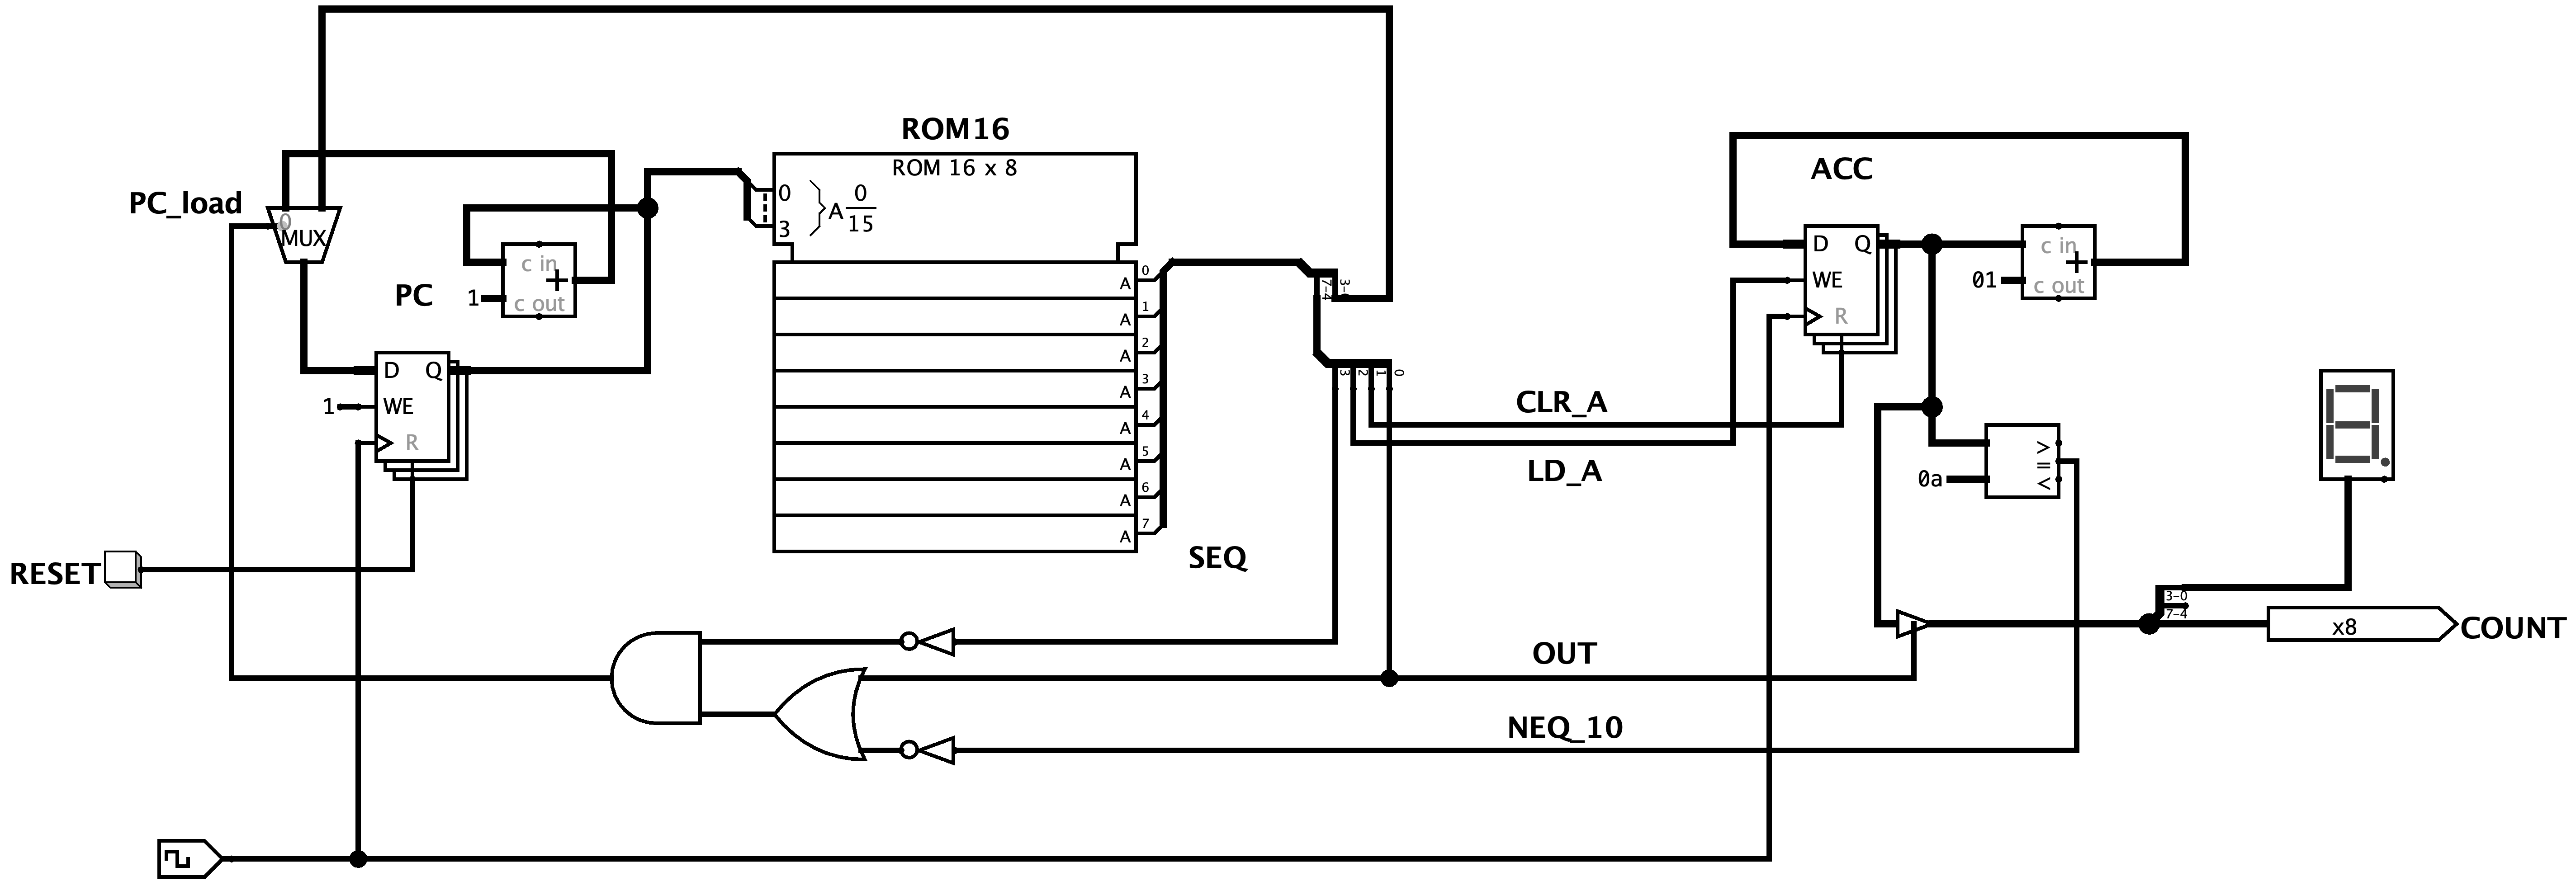
\includegraphics[width=\textwidth]{../assets/full-circuit.png}
\caption{The reference circuit. Left: \texttt{PC\_load} selects the \texttt{MUX}
feeding \texttt{PC}'s D input, either from the \texttt{+1} adder (constant
\texttt{1}) or looped back from \texttt{ROM16}'s own low nibble; \texttt{PC}
addresses \texttt{ROM16} directly (no MAR). Centre: \texttt{ROM16} (16$\times$8)
splits its output into \texttt{SEQ}, \texttt{CLR\_A}, \texttt{LD\_A}, \texttt{OUT}
and the 4-bit jump address fed back to the \texttt{MUX}. Right: \texttt{ACC} is a
register with its own \texttt{+1} adder (constant \texttt{01}) feeding back into
its D input, a comparator against constant \texttt{0a} (hex \texttt{0x0A}\,=\,10)
producing \texttt{NEQ\_10}, and a tri-state buffer gated by \texttt{OUT} driving
the 8-bit \texttt{COUNT} bus and a 7-segment display. Bottom: the AND/OR glue
logic computing \texttt{PC\_load}, plus \texttt{RESET} and the \texttt{Clock}.}
\label{fig:circuit}
\end{figure}

\subsection*{The Microprogram: Count 0 to 10}

\begin{center}
\begin{tabular}{@{}clccccc c@{}}
\toprule
\textbf{Addr} & \textbf{Meaning} & \texttt{SEQ} & \texttt{LD\_A} & \texttt{CLR\_A} & \texttt{OUT} & \texttt{ADDR} & \textbf{Hex} \\
\midrule
0 & Clear \texttt{ACC}              & 1 & 0 & 1 & 0 & 0000 & \texttt{0xA0} \\
1 & Output \texttt{ACC}             & 1 & 0 & 0 & 1 & 0000 & \texttt{0x90} \\
2 & Increment \texttt{ACC}          & 1 & 1 & 0 & 0 & 0000 & \texttt{0xC0} \\
3 & Wait (no-op)                 & 1 & 0 & 0 & 0 & 0000 & \texttt{0x80} \\
4 & Jump to 1 if \texttt{ACC}$\,\neq 10$ & 0 & 0 & 0 & 0 & 0001 & \texttt{0x01} \\
5 & Jump to self, keep outputting & 0 & 0 & 0 & 1 & 0101 & \texttt{0x15} \\
\bottomrule
\end{tabular}
\end{center}

\noindent\textbf{Before you build anything:} using the \texttt{PC\_load} equation
from the summary box, trace what happens at address 4 (\texttt{SEQ=0}) when
\texttt{ACC}$\,\neq 10$, and separately when \texttt{ACC}$\,=10$. Then trace
address 5: why, once reached, does the machine loop on itself \emph{forever}
regardless of \texttt{NEQ\_10}?

\subsection*{Quick Experiments (Try It)}

\begin{tryit}{PC jump mux, in isolation}
Build just the left portion of Figure~\ref{fig:circuit} (\texttt{PC}, its
\texttt{+1} adder, the \texttt{MUX} -- feed
\texttt{ADDR} and \texttt{PC\_load} from switches, not yet from ROM).
\begin{enumerate}[nosep,leftmargin=*]
  \item With \texttt{PC\_load=0}, does \texttt{PC} count up on every clock edge?
  \item Poke \texttt{ADDR=0101} and set \texttt{PC\_load=1}. What is \texttt{PC}
        after the next clock edge? What if you leave \texttt{PC\_load=1} and keep
        clocking?
\end{enumerate}
\end{tryit}

\begin{tryit}{Accumulator + comparator, in isolation}
Build just the right-hand portion of Figure~\ref{fig:circuit} (\texttt{ACC}, its
\texttt{+1} adder, the comparator against \texttt{0a}, and the tri-state buffer --
feed \texttt{LD\_A}, \texttt{CLR\_A}, \texttt{OUT} from switches).
\begin{enumerate}[nosep,leftmargin=*]
  \item Clear \texttt{ACC}, then clock \texttt{LD\_A=1} ten times. Does
        \texttt{NEQ\_10} go low exactly when \texttt{ACC} reaches \texttt{1010}?
  \item With \texttt{OUT=0}, does the \texttt{COUNT} bus show anything? What does
        Logisim display for a tri-state buffer's output when disabled?
\end{enumerate}
\end{tryit}

\begin{tryit}{The glue logic alone}
Build \texttt{PC\_load} $= \overline{\texttt{SEQ}} \cdot (\texttt{OUT} +
\texttt{NEQ\_10})$ from an AND gate and an OR gate, driven by three switches
(\texttt{SEQ}, \texttt{OUT}, \texttt{NEQ\_10}). (The reference circuit doesn't use
a separate NOT gate at all -- it negates the \texttt{SEQ} input pin directly on
the AND gate. Try building it that way too.)
\begin{enumerate}[nosep,leftmargin=*]
  \item Fill in all 8 rows of its truth table by hand, then check every row against
        your circuit.
  \item Which single input, if you don't know the other two, tells you the most
        about whether \texttt{PC\_load} will be 1?
\end{enumerate}
\end{tryit}

\section*{In-Lab Exercises (target: 2 hours)}

\begin{labexercise}{PC side \hfill {\small \itshape (25 min)}}
Build the left portion of Figure~\ref{fig:circuit} in full: the 4-bit \texttt{PC}
register (\texttt{WE} tied to constant \texttt{1}, so it latches every clock
edge; \texttt{R} from \texttt{RESET}), its \texttt{+1} adder, and the
\texttt{MUX}. Wire \texttt{PC}'s output directly to where \texttt{ROM16}'s
address will go.
\end{labexercise}

\begin{labexercise}{Accumulator side \hfill {\small \itshape (30 min)}}
Build \texttt{ACC}: the 4-bit register (\texttt{WE}\,=\,\texttt{LD\_A},
\texttt{R}\,=\,\texttt{CLR\_A}), its own \texttt{+1} adder feeding back into its
D input, a tri-state output buffer, and a comparator against constant
\texttt{0a} (\texttt{0x0A}\,=\,10) producing \texttt{NEQ\_10}.
\end{labexercise}

\begin{labexercise}{ROM16 and the control word \hfill {\small \itshape (20 min)}}
Add a 16 $\times$ 8-bit \textbf{ROM} (\texttt{ROM16}), addressed by \texttt{PC}.
Split its 8-bit output into \texttt{SEQ}, \texttt{CLR\_A}, \texttt{LD\_A},
\texttt{OUT} (1 bit each) and the 4-bit jump address using a Splitter. Wire the
three \texttt{ACC} control bits straight to Exercise 2's circuit, and the jump
address straight to Exercise 1's \texttt{MUX} input \texttt{1}.
\end{labexercise}

\begin{labexercise}{The glue logic \hfill {\small \itshape (15 min)}}
Build \texttt{PC\_load} $= \overline{\texttt{SEQ}} \cdot (\texttt{OUT} +
\texttt{NEQ\_10})$ from Try It 3, and wire it to the \texttt{MUX}'s select
input. This is the \emph{entire} control unit for this machine -- notice there is
no state register anywhere in it.
\end{labexercise}

\begin{labexercise}{Assemble, load, and run \hfill {\small \itshape (30 min)}}
Wire Exercises 1--4 together exactly as in Figure~\ref{fig:circuit}, with a
\texttt{Button} for \texttt{RESET}, a \texttt{Clock}, and a \texttt{HexDisplay}
on \texttt{COUNT}. Hand-assemble the microprogram from the table above and load
it into \texttt{ROM16} with \emph{Load Image}:
\begin{lstlisting}
v2.0 raw
a0 90 c0 80 01 15 00 00 00 00 00 00 00 00 00 00
\end{lstlisting}
Single-step the clock and confirm: \texttt{COUNT} shows \texttt{0, 1, 2,
\ldots, 10} in turn, one value per pass through address 1, and then the machine
settles at address 5, continuously re-displaying \texttt{10} forever.
$\square$~Count sequence matches. $\square$~Machine settles at address 5 (watch
\texttt{PC} stop advancing past 5).
\end{labexercise}

\begin{aicollab}
\textbf{Try these prompts with an AI tool:}
\begin{itemize}[leftmargin=*,nosep]
  \item ``What is the architectural difference between a machine where the ROM
        word is decoded by an FSM, versus one where the ROM word directly drives
        the datapath?''
  \item ``Given \texttt{PC\_load = NOT(SEQ) AND (OUT OR NEQ\_10)}, is there a
        smaller circuit that computes the same function?''
  \item ``What Logisim-Evolution component implements a 4-bit magnitude
        comparator, and how do I wire one input to a fixed constant?''
\end{itemize}

\medskip\textbf{Critical check -- verify, don't just accept:}
Ask the AI whether this machine's control unit qualifies as a ``Moore machine,''
a ``Mealy machine,'' both, or neither. Then justify the answer yourself, in
writing, from the actual circuit -- \texttt{PC\_load} depends combinationally on
\texttt{NEQ\_10}, which itself depends on the \emph{current} value of a register
(\texttt{ACC}), not on any external input. Does that change the classification
the AI gave you?

\medskip\textbf{Know the limit:}
AI tools often default to describing microprocessors in terms of
fetch/decode/execute because that is the overwhelmingly common case in their
training data. This machine has no decode stage at all -- if you ask a leading
question (``how does this machine decode its opcode?''), many models will
happily invent a decode step that doesn't exist here rather than telling you the
premise is wrong.
\end{aicollab}

\takehomebanner

\begin{trace}[Six clock cycles from reset]
Assume \texttt{PC} resets to 0. Fill in a table with columns \emph{Cycle, PC,
Control word (hex), ACC, COUNT} for the first six clock edges. At which cycle
does \texttt{COUNT} first show a nonzero value?
\end{trace}

\begin{bug}[A swapped mux input]
A student wired \texttt{ROM16}'s jump-address field into the \texttt{MUX}'s
input \texttt{0} and the \texttt{+1} adder into input \texttt{1} (i.e.\ the two
mux inputs from Figure~\ref{fig:circuit} are swapped), but the \texttt{PC\_load}
equation is otherwise correct and unchanged. Predict exactly what \texttt{PC}
does starting from address 0, for at least the first 8 cycles. Does the machine
still count correctly?
\end{bug}

\begin{writecode}[Design a count-down microprogram]
Using the same control-word format, write a new 16-word microprogram that counts
\emph{down} from 10 to 0 (instead of up), still outputting every value and
settling into a self-loop at 0. You will need a different comparator target
(\texttt{NEQ\_0}, i.e.\ \texttt{ACC}$\,\neq 0$) and a decrementer instead of an
incrementer. Write out the full table (address, mnemonic meaning, all five
control fields, hex) as in the Quick Reference above.
\end{writecode}

\begin{drawex}{Control-word datapath, from memory}
Without looking at Figure~\ref{fig:circuit}, draw the complete datapath from
memory: \texttt{PC}, its \texttt{+1} adder, the \texttt{MUX}, \texttt{ROM16},
the Splitter's five output fields, \texttt{ACC}, its own \texttt{+1} adder, the
tri-state buffer, the comparator, and the glue logic feeding the \texttt{MUX}'s
select line. Compare against the real figure afterward and mark anything you
got wrong or omitted.
\end{drawex}

\end{document}
